\documentclass[12pt]{article}
\usepackage{graphicx}
\graphicspath{{Images/}}
\usepackage{textcomp} %for the copywrite symbol
%\linespread{1.6} %sets lines to 1.5 spacing.  1.6 would be double spaced
\usepackage[margin=1.0in]{geometry}
\usepackage[semicolon,round,sort&compress,sectionbib,numbers]{natbib}  
\usepackage{chapterbib}  
\usepackage{amsmath}
\usepackage{subcaption}
\usepackage{appendix} %for appendices
\usepackage{float}
\usepackage{listings}

\usepackage{hyperref} %make stuff clickable
\hypersetup{
	colorlinks,
	citecolor=black,
	filecolor=black,
	linkcolor=black,
	urlcolor=black
}


\usepackage{physics}  %for bras and kets!
\newcommand{\angstrom}{\mbox{\normalfont\AA }} %makes \angstrom do its thing!

\title{Lithium Diffusion with Quantum Espresso and ATAT}

\begin{document}
\maketitle

\tableofcontents


\section{Tools you'll need}

\begin{itemize}
	\item Quantum Espresso (QE)/similar DFT code capable of NEB
	
	\item ATAT for cluster expansion
	
	\item VESTA/Xcrysden for structure visualization 
	
	\item Coding language of choice to write Monte Carlo simulation
\end{itemize}

\section{Procedure}

There are three main steps to performing a Kinetic Monte Carlo (KMC) simulation:
\begin{itemize}
	\item  Obtaining activation barriers through Nudged Elastic Band (NEB) method 
	\item  Performing a cluster expansion to generalize the barriers to all possible configurations
	\item Using the activation barriers to perform a Monte Carlo simulation.
\end{itemize}


\section{Activation Barriers}
The activation barrier is the energy required to move an electron from one lattice site to another, and is a fundamental property defining diffusion rates.  Practically it can be obtained from DFT through the Nudged Elastic Band (NEB) method.  This method inherently requires quite large unit/super cells, running a large number of ground state calculations, and only depends on the ground state energy of the system.  As such, a Pseudo-potential code such as VASP or QE is an appropriate choice over more computationally heavy all electron options (Wien2k, exciting).  \\




\subsection{Quantum Espresso}
Quantum espresso is a DFT code that can be used to calculate activation barriers through the  nudged elastic band method. It can be relatively easy to install,  download the source code from \url{https://github.com/QEF/q-e/releases}, and extract it to an appropriate directory (eg. ~/Programs).  Then \textbf{\$ ./configure} and \textbf{\$ make all} should run cleanly as indicated in the readme.  Fianlly, add the quantum espresso bin directory to your path, by adding something like the following to your .bashrc file:

\begin{lstlisting}
export PATH=$PATH:path-to-qe-install/qe-6.3/bin
\end{lstlisting}

\subsubsection{NEB calculation}
The main features of quantum espresso are well explained in the documentation and tutorials.  the reader should use these to become accustomed to perform standard convergence tests (k points, ecut, mixing beta, smearing, etc.). It is essential to use converged parameters for the NEB calculating to obtain the correct path.  

NEB works by calculating the energy and forces acting on a single atom in the crystal at various points along a path between two neighbouring lattice sites. By minimizing the forces normal to the path, the lowest energy path can be found.  Some degree of force along the path is also taken into consideration to keep the path length short, giving rise to the ``elastic band" nature of this technique.   

Again this procedure is well explained in the documentation, which can be found here: \url{https://www.quantum-espresso.org/Doc/neb_user_guide.pdf}, along with examples in the /qe-\#\#/NEB/Examples directory.  

NEB paths can be visualized and animated using Xcrysden by calling the --xsf flag:  \textbf{\$ xcrysden --xsf case\_name.axsf }.  

\section{ATAT/Cluster Expansion}

The cluster expansion is the key step in being able to scale the atomic level properties to the bulk.  It allows for the activation barrier to be rapidly computed for any general configuration of a supercell.  Rapidly in this case means based on addition and multiplication and not a full dft calculation.  \\

It is also the hardest part of this process conceptually to understand, so I will run through a basic example here. The aim of the cluster expansion is to be able to return the groundstate energy of the system given a random configuration.  eg:\\
\begin{figure}[H]
	\centering
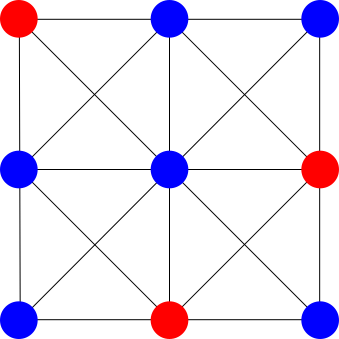
\includegraphics[scale=0.5]{./images/config.png}
\caption*{Energy = -77 eV}
\end{figure}

Where the red and blue spheres correspond to different atoms/vacancies.  \\

As, even in this simple example (2 atom types, 9 locations) there are $2^9 = 512$ possible configurations, it is impractical to calculate and save the groundstate for each one through DFT.   The solution to this is to instead calculate the effective cluster interaction (ECI's) for the crystal, which can be typically done using ``only" dozens of calculations.   What are ECI's?  They are the energies associated with the occupancy of each cluster in the structure. 
We will start by considering the simplest case and work up from there.  The simplest case is no dependence on occupancy, the zeroth order term, which can be thought of as the energy of the all the other atoms in the crystal.  In this case: 


\begin{figure}[H]
	\centering
	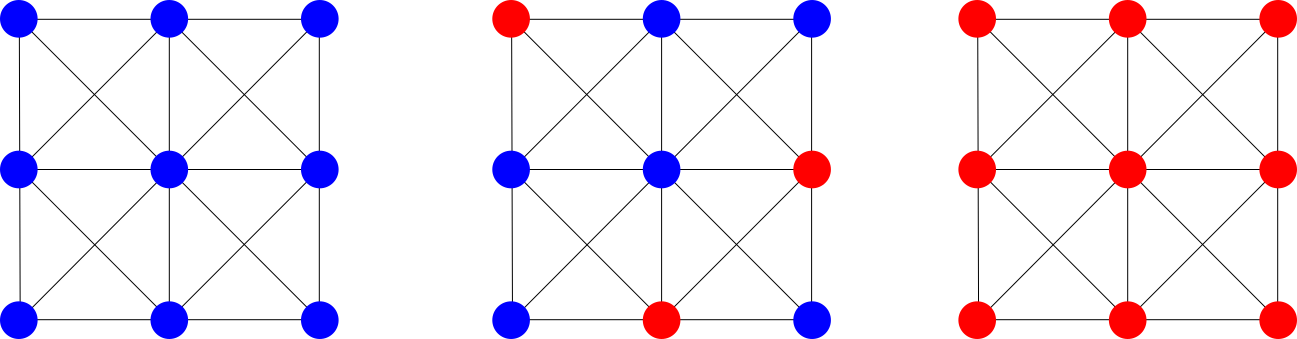
\includegraphics[scale=0.5]{./images/triplet.png}
	\caption*{Energy all cases = $\epsilon_0$ = -50 eV}
\end{figure}

This is obviously not very accurate, so to improve upon this method, we consider the single atom clusters.  To do this, we assign a value to each site depending on which atom occupies it: $n_i=$ -1 or a 1. The total energy then becomes: 

\[
E = \epsilon_0 + \epsilon_1 (n_1 + n_2 +n_3 + \dots + n_N )
\]


\begin{figure}[H]
	\centering
	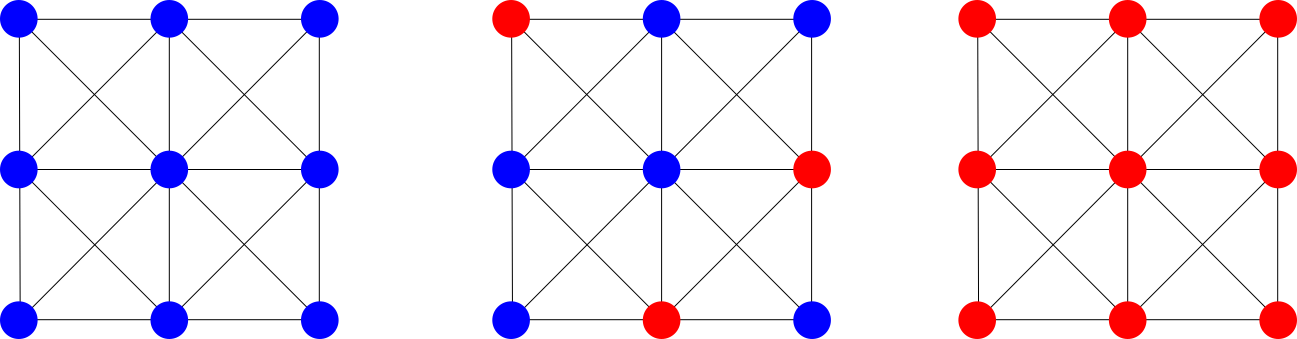
\includegraphics[scale=0.5]{./images/triplet.png}
	\caption*{$E_1 =-50eV + (1eV)(9) = -41 eV$, $E_2 = -50eV+ (1eV)(3) = -47eV$, $E_3 = -50 eV + (1eV)(-9) = -59eV$}
\end{figure}

This is a definite improvement, but the real benefit of the cluster expansion is in detecting the effects of long range ordering, ie in differentiating between cases such as:

\begin{figure}[H]
	\centering
	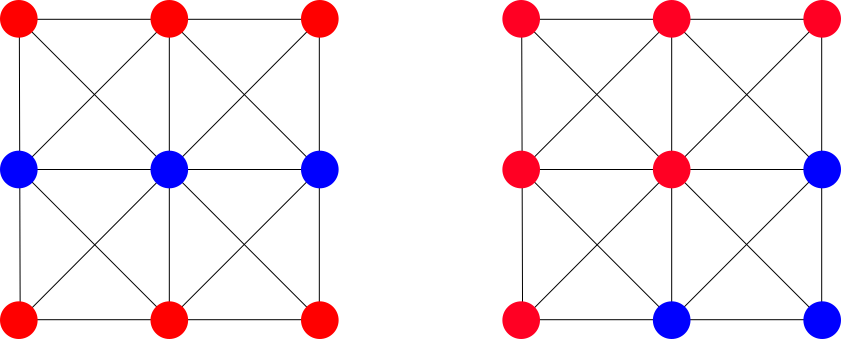
\includegraphics[scale=0.5]{./images/ordered.png}
	\caption*{Want $E_1\neq E_2$}
\end{figure}

To obtain this kind of accuracy, we need to include higher order terms, starting with 2 atom clusters.  We start by considering the ECI from adjacent atoms. The trick is in not double counting any clusters, so as we cycle through each site we only consider two and not four pairs:  

\begin{figure}[H]
	\centering
	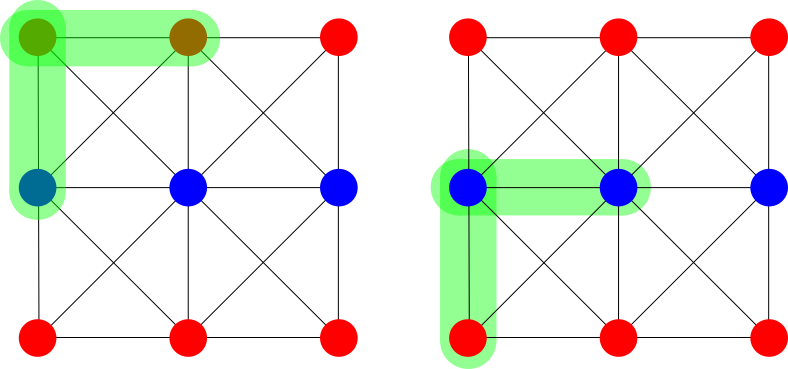
\includegraphics[scale=0.5]{./images/doublets.png}
	\caption*{The two clusters considered for each atom}
\end{figure}

Adding these to the single clusters makes the total energy: 

\[
E = \epsilon_0 + \epsilon_1 (n_1 + n_2 +n_3 + \dots + n_N ) + \epsilon_2 \bigg[(n_1n_2 + n_1n_4) + (n_2n_3 + n_2n_5) + \dots + (n_9n_1+n_9n_3)\bigg]
\]


In this case we assume ordering through the periodic boundaries, which may or may not be what is wanted. This is not the only two atom cluster that can be considered, an ECI can be calculated for any two atoms in the cell.  However, ECI's tend to be inversely proportional to the distance between atoms in the cluster, and often the nearest, and next nearest neighbours are sufficient.  ECI can also be calculated for triplets and quadruplets as well, but ECI's also tend to decrease with increasing cluster size.  Depending on cell size and desired accuracy, a typical cluster expansion might include anywhere between 5-20 ECI's, which will typically include 3-7 doublts,3-10 triplets, and maybe a couple quadruplets.  \\

\subsection{How to Calculate ECI's}
ECI's are calculated by running a subset of the configurations and obtaining the groundstate energies.  At this point, the ECI's can be determined by optimizing the total energy calculation to produce these values.  To avoid divergence, this requires at minimum one more calculation than the number of ECI's. Selecting which configurations to calculate to converge the cluster expansion fastest is what ATAT does, as well as calculating the ECI on the fly and providing convergence estimates.  \\

\subsection{Local Cluster Expansion}
In the case of diffusion however, the value we care about is the activation barrier, which complicates the situation.  Performing 50+ NEB calculations would be immensely time consuming.  The solution is to determine the minimum energy pathway and perform cluster expansion calculations for two cases in each configuration, one in the groundstate and one where the moving atom is located at the high point of this pathway.  Subtracting these energies gives an estimate of the activation energy, which is now the value that the ECI's can be fit to.  \\

This method dramatically increases the number of ECI's necessary as the symmetry of the cell has been broken, and each site needs to be treated individually.  The activation energy calculation might then look something like this:

\[
E_{act} = \epsilon_0 + \epsilon_1 n_1 + \epsilon_1^2 n_2 + \epsilon_1^3 n_3 + \dots + \epsilon_2 n_1n_2 +\epsilon_2^2 n_1n_3 + \epsilon_2^3 n_2n_4 + \dots
\]



\section{KMC}
Once the ECI of a local cluster expansion have been determined, it is possible to increase the length scale again to obtain bulk diffusion properties, through Monte Carlo.  This procedure is well documented in Van der Ven and Ceder's paper.  



\end{document}